%%%%%%%%%%%%%%%%%% USAGE INSTRUCTIONS %%%%%%%%%%%%%%%%%%
% - Compile using LuaLaTeX and biber, unless there is a particular reason not to. Do not use the older LaTex/PDFLaTeX or BibTeX. (The fonts won't work correctly.)
% - Font and the report 'year' must be specified when all \documentclass or the template won't work correctly. (There's no error checking/default cases!)
% - For best performance save images/graphics as PDF files, not as png/jpg/eps. This makes no difference to how images are inserted using \includegraphics.
% - As many further packages as wanted can be loaded. Below are just an example set. Note that template itself loads a number of packages, including hyperref.
% - References are handed using biblatex.
% - Link to the presentation of theses policy: https://documents.manchester.ac.uk/DocuInfo.aspx?DocID=2863

%%%%%%%%%%%%%%%%%% META DATA SETUP %%%%%%%%%%%%%%%%%%
% This is where the document title and author are set. Other details for the title page are set later
% Note that if/when you edit these you may need to 'Recompile from scratch' to get the changes to display in the PDF. (In Overleaf, select the down arrow to the right of the 'Recompile' button)
\begin{filecontents*}{\jobname.xmpdata}
    \Title{Development of Two Wheel Self Balancing Platform for Monocular Vision Based Trajectory Tracking} % title of your thesis
    \Author{Winston Scott 107067151} % should be student number rather than name to help with annoymous marking
    \Language{en-GB}
    \Copyrighted{True}
    % More meta-data fielda can be added here if wanted, see https://ctan.org/pkg/pdfx?lang=en for fields
  \end{filecontents*}
  %%%%%%%%%%%%%%%%%% DOCUMENT SETUP %%%%%%%%%%%%%%%%%%
  \documentclass{uom_eee_dissertation_casson} 
  %%%%%%%%%%%%%%%%%% PACKAGES AND COMMANDS %%%%%%%%%%%%%%%%%%
  % Packages
  \usepackage{graphicx,psfrag,color} % for postscript graphics files
    \graphicspath{ {./DesingImgs/} }
  \usepackage{amsmath}               % assumes amsmath package installed
    \allowdisplaybreaks[1]           % allow eqnarrays to break across pages
  \usepackage{amssymb}               % assumes amsmath package installed 
  \usepackage{url}                   % format hyperlinks correctly
  \usepackage{rotating}              % allow portrait figures and tables
  \usepackage{multirow}              % allows merging of rows in tables
  \usepackage{lscape}                % allows pages to be typeset in landscape mode
  \usepackage{tabularx}              % allows fixed width tables
  \usepackage{verbatim}              % enhanced version of built-in verbatim environment
  \usepackage{footnote}              % allows more control over footnote environments
  \usepackage{float}                 % allows H option on floats to force here placement
  \usepackage{booktabs}              % improve table line spacing
  \usepackage{lipsum}                % for adding dummy text here
  \usepackage[base]{babel}           % for proper hypthenation in lipsum sections
  \usepackage{subcaption}            % for multiple sub-figures in a single float
  % Add your packages here
  %\usepackage{pdfcomment}            % for alt text for accessibility
  % Then to add images use:
  % \pdftooltip{\includegraphics[width=0.5\textwidth]{image.pdf}}{Alt-text here}
  % This makes the text in the image non-select-able though (assuming it's a vector file)
  
  % Custom commands
  \newcommand{\degree}{\ensuremath{^\circ}}
  \newcommand{\sus}[1]{$^{\mbox{\scriptsize #1}}$} % superscript in text (e.g. 1st)
  \newcommand{\sub}[1]{$_{\mbox{\scriptsize #1}}$} % subscript in text
  \newcommand{\sect}[1]{Section~\ref{#1}}
  \newcommand{\fig}[1]{Fig.~\ref{#1}}
  \newcommand{\tab}[1]{Table~\ref{#1}}
  \newcommand{\equ}[1]{(\ref{#1})}
  \newcommand{\appx}[1]{Appendix~\ref{#1}}
  %%%%%%%%%%%%%%%%%% REFERENCES SETUP %%%%%%%%%%%%%%%%%%
  % Setup your references here. Change the reference style here if wanted
  \usepackage[style=ieee,backend=biber,backref=true,hyperref=auto]{biblatex}
  % Note backref=true adds a page number (and hyperlink) to each reference so you can easily go back from the references to the main document. You may prefer backref=false if you need to stick strictly to a given reference style
  % Fixes which can't be applied in the .cls file
  \DefineBibliographyStrings{english}{backrefpage = {cited on p\adddot},  backrefpages = {cited on pp\adddot}}
  %  \renewcommand*{\bibfont}{\large}
  % Add more .bib files here if wanted
  \addbibresource{references.bib}
  
  %%%%%%%%%%%%%%%%%% START DOCUMENT %%%%%%%%%%%%%%%%%%
  % Don't edit these lines, title and author are automatically taken from the document meta-data defined above
  \begin{document}
  \makeatletter
  \title{\xmp@Title}
  \studentid{\xmp@Author}
  \makeatother
  
  % Set the below yourself
  \course{Mechatronics and Robotics Engineering}  % "Master of Science in" is added automatically
                                                     % Our courses are: Advanced Control and Systems Engineering, Advanced Control and Systems Engineering with Extended Research, Communications and Signal Processing, Communications and Signal Processing with Extended Research, Electrical Power Systems Engineering, Advanced Electrical Power Systems Engineering, Renewable Energy and Clean Technology, Renewable Energy and Clean Technology with Extended Research
  \submitdate{2025}                                  % regulations ask only for the year, not month
  \wordcount{1000}		                            % use \wordcount{} to set the count, \thewordcount to print in the text
  \maketitle

  %%%%%%%%%%%%%%%%%% LISTS OF CONTENT %%%%%%%%%%%%%%%%%%
  \uomtoc
  % other lists are not required, but can include \uomlof and \uomlot if really want to

  %%%%%%%%%%%%%%%%%% ABSTRACT %%%%%%%%%%%%%%%%%%
  \begin{abstract} % put abstract here. Limit is 1 page.
    Abstract goes here.
  \end{abstract}%
  \clearpage
  %%%%%%%%%%%%%%%%%% SECTION 1 %%%%%%%%%%%%%%%%%%
  \section{Introduction}
    \subsection{Background and motivation}
    \subsection{Aims and objectives}
  %%%%%%%%%%%%%%%%%% SECTION 2 %%%%%%%%%%%%%%%%%%
  \section{Literature review} % edit section heading as appropriate

    \subsection{Introduction}

    This is now a MIMO control problem. numerous control strategies have been used to solve this problem, 
    with different goals in mind. [dadsasd] presents a lqr controller which tracks 
    the desiered velocity, leanding itself to telleorative usecases, [sadasda] 
    shows how a casscasded PID controlleri is used to perform postion control, 
    and [aasdasd] explores how a nerual net can be used for swing up and balance control.
    \subsection{Summary}
  %%%%%%%%%%%%%%%%%% SECTION 3 %%%%%%%%%%%%%%%%%%
  \pagebreak{}
  \section{Methodology } % edit section heading as appropriate
  \subsection{Dynamic Model}
    \includegraphics[width=\textwidth]{ModelingDiags.pdf}

    \subsection{System Design}
        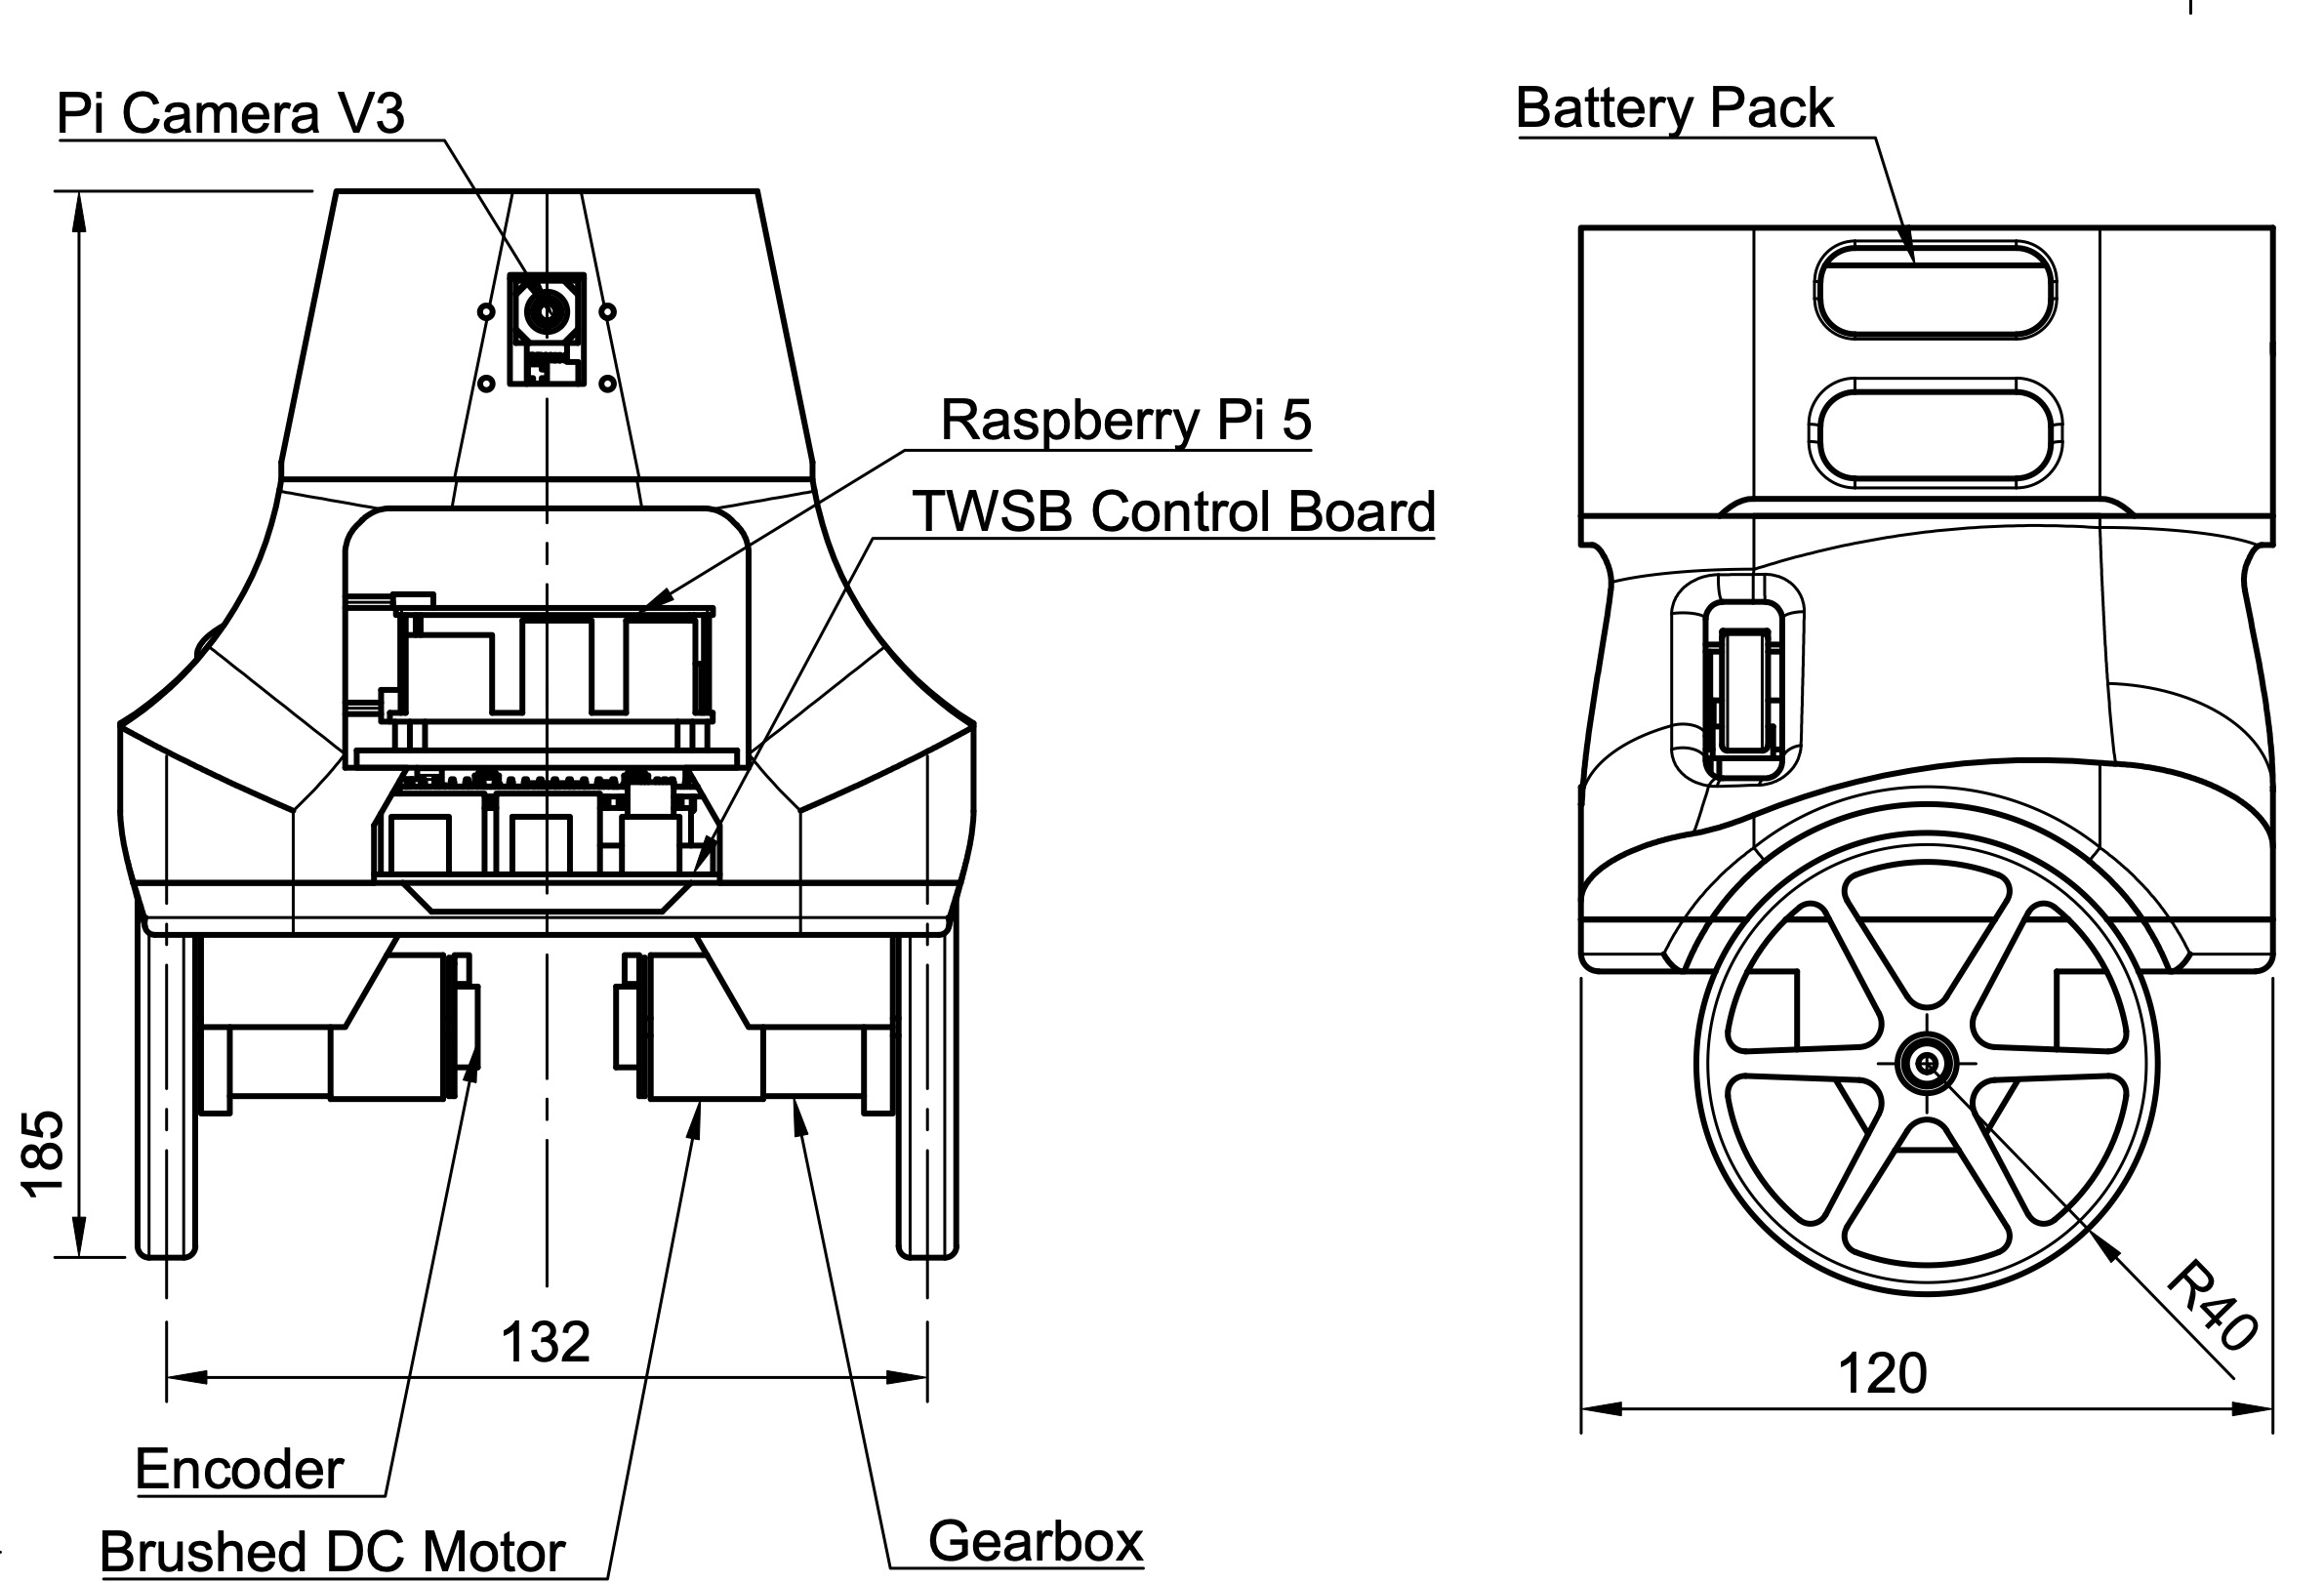
\includegraphics[width=\textwidth]{bBotV2TechDraw.pdf}
        The TWSB is printed out of PLA plastic in 3 parts for minimal assembly.
        The battery pack is quickly swappable and both it and the electronics section 
        are soft-mounted in a roll cage like for protection against impacts. 
        
        \includegraphics[width=\textwidth]{SystemOverview.pdf}

        \subsubsection{Parameters}

        \subsection{Software Architecture}
        \subsubsection{Compute Systems Overview }
        \includegraphics[width=\textwidth]{CommunicationDataPath.pdf}  
            The software system is managed as systemd services.
            Programs implement a runtime GET/SET/RUN rpc interface,
            this significantly reduces iteration time and separates 
            complex and fallible processes like the Gstreamer pipeline 
            from the main control loop. 
            A Gstreamer pipeline setup a RSTP server which can be accessed on the network.

        \includegraphics[width=\textwidth]{FirmwareArch.pdf}
            The Firmware is implemented in c99 using the libopencm3 project[].
            The MCU also presents the same rpc ascii interface over serial. 
            The super-loop executes commands at 10Hz, 
            and publishes its state at 100Hz.


        

    \subsection{State Estimation}
        \subsubsection{Parameter Estimation}
        \subsubsection{Sensors Overview}
        \subsubsection{Kalman Filter}
        \subsubsection{Extended Kalman Filter}
    \subsection{Control System}
       
        A simple PD controller is often enough to stabilize one of the systems dynamic variables c[].
        However as shown by fig3, x position drifts. Since the linear velocity is coupled to the
        pitch angle by eq(1), the pitch angle must be controlled to maintain a constant x velocity. 
       
        The navigation algorithms discussed in section 3.7 require the 
        TWSB to present a layer of abstraction enabling the platform to be modeled as a point G in 2D plane 
        as shown in fig. 3. 

        \subsubsection{Cascade PID}
        A cascaded pid controller is used to control the pitch angle and the linear velocity.
        A P controller is used to regulate the steering control signal, which modded
        as a disturbance from the 2D dynamics model. 
        \subsubsection{LQR}
        The TWSB robot is a MIMO system, using the state space representation of the system in eq[1]
        



        \subsubsection{Reference Tracking}

 

    \subsection{Vision System}
        \subsubsection{Curvilinear Transformation}
        The planar two wheel self balancing robot, now modeled as a point P, subject to the differential drive constraints, 
        can be instantaneously described as following some segment or radius r. This arc seggment forms part of a coninuous spline. 
        The curvature of the spline is given by the inverse of the radius of the circle that best fits the arc segment.
        Where a positive curvature indicates a right turn and a negative curvature indicates a left turn.
        The forward direction is x, and left if y. using the side of the angle between the robtos heading and the observed center line can be used as the derivative term.
        adding the curvature K, 
            \subsubsection{Pipeline}
            \subsubsection{Camera Calibration}
            \subsubsection{IMU Based Software Stabilization Methods}
            \subsubsection{Perspective Transformation}
            \subsubsection{Polynomial Fitting}
            \subsubsection{Trajectory Generation}


  %%%%%%%%%%%%%%%%%% SECTION 4 %%%%%%%%%%%%%%%%%%
  \section{Results and discussion} % edit section heading as appropriate
    \subsection{Introduction}
    \subsection{Balance Performance}
    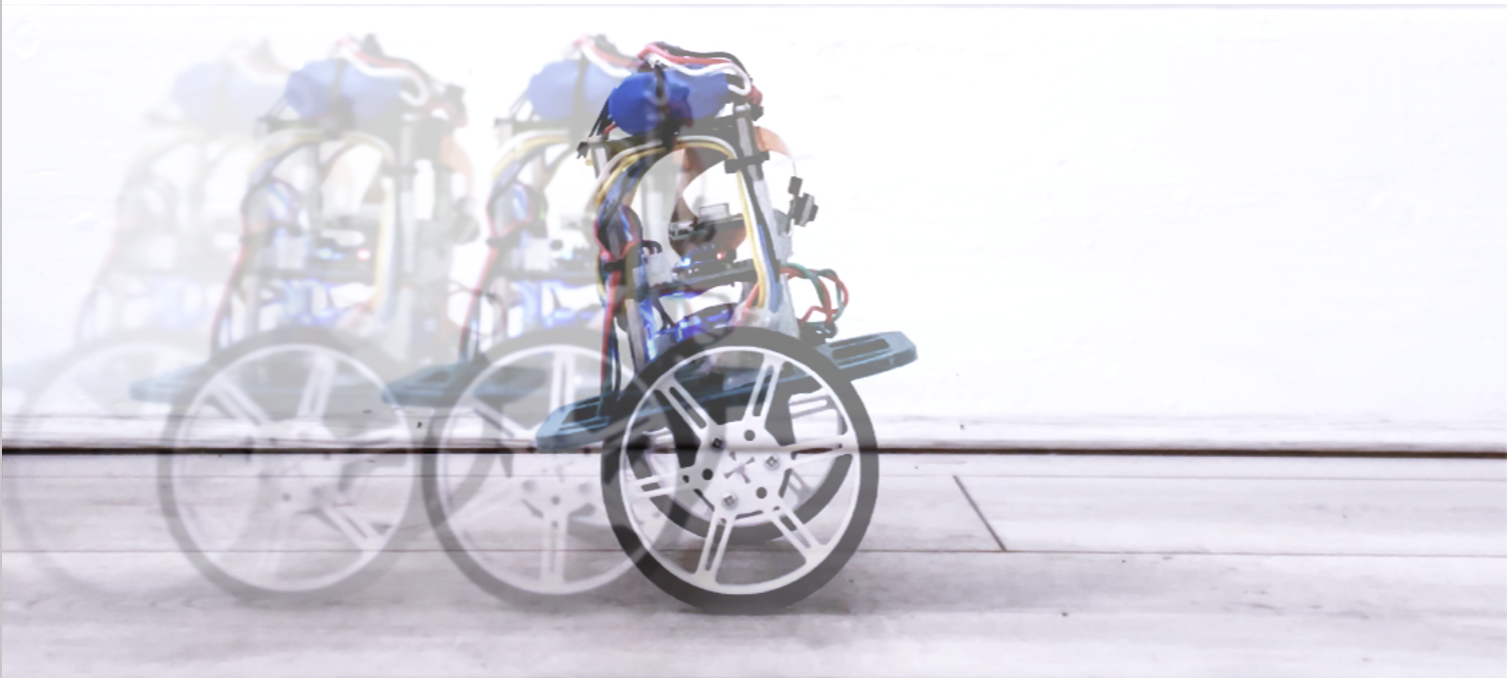
\includegraphics[width=\textwidth]{V1Colated.png}
    \subsection{Operational Robustness}
    \subsection{Line Trajectory Tracking}
    \subsection{More detail}
    \subsection{Summary}
  %%%%%%%%%%%%%%%%%% SECTION 5 %%%%%%%%%%%%%%%%%%
  \section{Conclusions and future work} % edit section heading as appropriate
    \subsection{Conclusions}
      \subsection{Future work}
  %%%%%%%%%%%%%%%%%% REFERENCES %%%%%%%%%%%%%%%%%%
  %\clearpage % uncomment to start on a new page if wanted
  \printbibliography[title={References},heading=bibintoc] % a single list of references for the whole thesis
  %%%%%%%%%%%%%%%%%% APPENDICES %%%%%%%%%%%%%%%%%%
  \begin{uomappendix} 
      \section{Code}
      \section{Risk assessment}
      Risk assessment is a required appendix. Put here.
      %\section{Other appendices as necessary}
  \end{uomappendix}
  
  %%%%%%%%%%%%%%%%%% END MATTER %%%%%%%%%%%%%%%%%%
  \end{document}